\chapter{Discussion \& perspectives}
{
\hypersetup{linkcolor=GREYDARK}
\minitoc
}

\section{Conclusion}

$\bullet$ Recall the frame and goals of the thesis (see chapter~\ref{chap:goals}).

$\bullet$ Mutational bias result in fixation bias in the other direction (which can be confounded with gBGC).

$\bullet$ By modeling fixation bias, mutational bias can be inferred reliably.

$\bullet$ It is possible to construct and implement models of evolution parameterized by drift across branch and selection across sites.

$\bullet$ There is persistent signal in substitution patterns that relates to past drift.

$\bullet$ However, assumptions on the properties of the fitness landscape, namely that each site is independent results in low sensitivity.

$\bullet$ Susceptibility of $\dnds$ to changes in $\Ne$ is between two extremes, site independent fitness landscapes, and phenotype define for the whole sequence.

\section{Epistasis and entrenchment}

$\bullet$ A blind spot of the mutation-selection phylogenetic codon model is the assumption of site-independence, each site is an independent Markov chain.

$\bullet$ Previous studies have argued that models of molecular evolution should consider the importance epistasis for its role in speciation, in modulating the rate of adaptation, and many other factors~\citep{Goldstein2017, Miller2018}.

$\bullet$ From a modeling and inference perspective, accounting for epistasis is challenging both in terms of parametrization and computational complexity~\citep{Rodrigue2005, Manhart2014}.

$\bullet$ I argue that epistasis also has an important role in the response of $\dnds$ to changes in $\Ne$, both in terms of susceptibility and dynamic of the response.

$\bullet$ Fundamentally, any model modeling fitness at the site level (without epistasis) implies a slow dynamic and a strong susceptibility, and adding epistasis to the model imply a faster dynamic and a weaker susceptibility.
Intuitively, this effect originates in the fact that each site is to adapt independently to changes in $\Ne$ leading to overall a slow response (substitutions must affect all sites), and a strong susceptibility since each site will change its position in the fitness landscape.
Taking into account epistasis, the burden of adapting to changes in $\Ne$ is shared by more sites, such that all of them don't have to switch position.

$\bullet$ On the other hand, entrenchment due to specific epistasis has implication in terms of the assumption of a static fitness landscape.
Fitness landscapes are considered static, where the current sequence is sitting on the high ground of the fitness landscape, where by high ground I mean that the gap between peaks and current sequence is on the order of $1 / \Ne$.
With epistasis, fitness landscape is not static but dynamic, and for a specific site the proposed mutations are mostly from high ground into a fitness valley, where such valley is getting deeper and deeper with time.
In other words the selection coefficient of proposed mutations are getting increasingly negative with time, mimicking a dynamic fitness landscape.

\section{Adaptive landscape}
\label{sec:adaptative-landscape}

$\bullet$ Another blind spot of the mutation-selection is the assumption of a static fitness landscape.

$\bullet$ With seascape, fitness landscape is not static but dynamic, and for a specific site the proposed mutations are mostly from high ground into a fitness valley.
Because of the movement of the landscape behind our feet, similarly to a Red-Queen dynamic, it is more likely to slide into a valley rather than on top of a peak when the landscape moving.
In other words, because the current sequence is at marginal stability, and that they are more ways to move downward that upwards in the fitness landscape, any changes of the landscape results in lower elevation of the current coordinate. The resulting dynamic is that selection pushes the sequence to climb up the landscape constantly.

$\bullet$ This effect translates into a discrepancy between $\omega$ and $\omega_0$, where $\omega > \omega_0$ is signature of adaption~\citep{Rodrigue2016}.
As a result, the assumption of static landscape can be turned into an advantage, where $\omega_0$ is the null model of absence of adaptive evolution, in the sens that the fitness landscape is not moving.
It is important to note that because of the mutation-selection-drift equilibrium is not optimized, their is always of proportion of advantageous mutation that are proposed.

$\bullet$ $\omega$ and $\omega_0$ can be estimated along the sequence, such that mutation-selection framework can detect site-specific adaptive evolution in protein-coding genes.
Such method has been implemented in Bayescode, and the manuscript is available in appendix page \pageref{sec-appendix:MutSelM3starMBE}.

$\bullet$ Moreover, contrasting $\omega$ and $\omega_0$ lead to estimation of the rate of adaptive substitution as:
\begin{equation}
    \omega_A = \omega - \omega_0
\end{equation}

$\bullet$ This phylogenetic estimation of the proportion of adaptation can be confronted to estimation of adaptation obtained with polymorphism dataset within species.
Originally pioneered by \citet{McDonald1991}, the ratio of non-synonymous over synonymous polymorphism ($\pnps$) supposedly solely contains non-adaptive polymorphism.
On the other hand, divergence data allows to estimate the ratio of non-synonymous over synonymous substitutions ($\dnds$), supposedly composed of a mixture of both advantageous substitutions and non-adaptive (nearly-neutral) substitutions.
Thus the difference $\dnds - \pnps $ is the rate of adaptive evolution.

$\bullet$ To note, the rate of non-adaptive evolution, $\pnps$ obtained with polymorphism data supposedly matches the compound parameters $\omega_0$ obtained uniquely from divergence data.

$\bullet$ However, estimation of adaptive rate can be biased by moderately deleterious mutations~\citep{eyre-walker_quantifying_2002} and by the change in population size through time~\citep{eyre-walker_changing_2002}.
To overcome this biases, the method of \citet{Galtier2016} relies on the synonymous and non-synonymous site-frequency spectra (SFS) to estimate the distribution of fitness effects of mutations (DFE), modeled as a continuous distribution.
Subsequent development of these methods are reviewed in~\citep{Moutinho2019a}, intrinsically measuring the rate of non-adaptive evolution present in polymorphism data.

\begin{figure}[H]
	\centering
	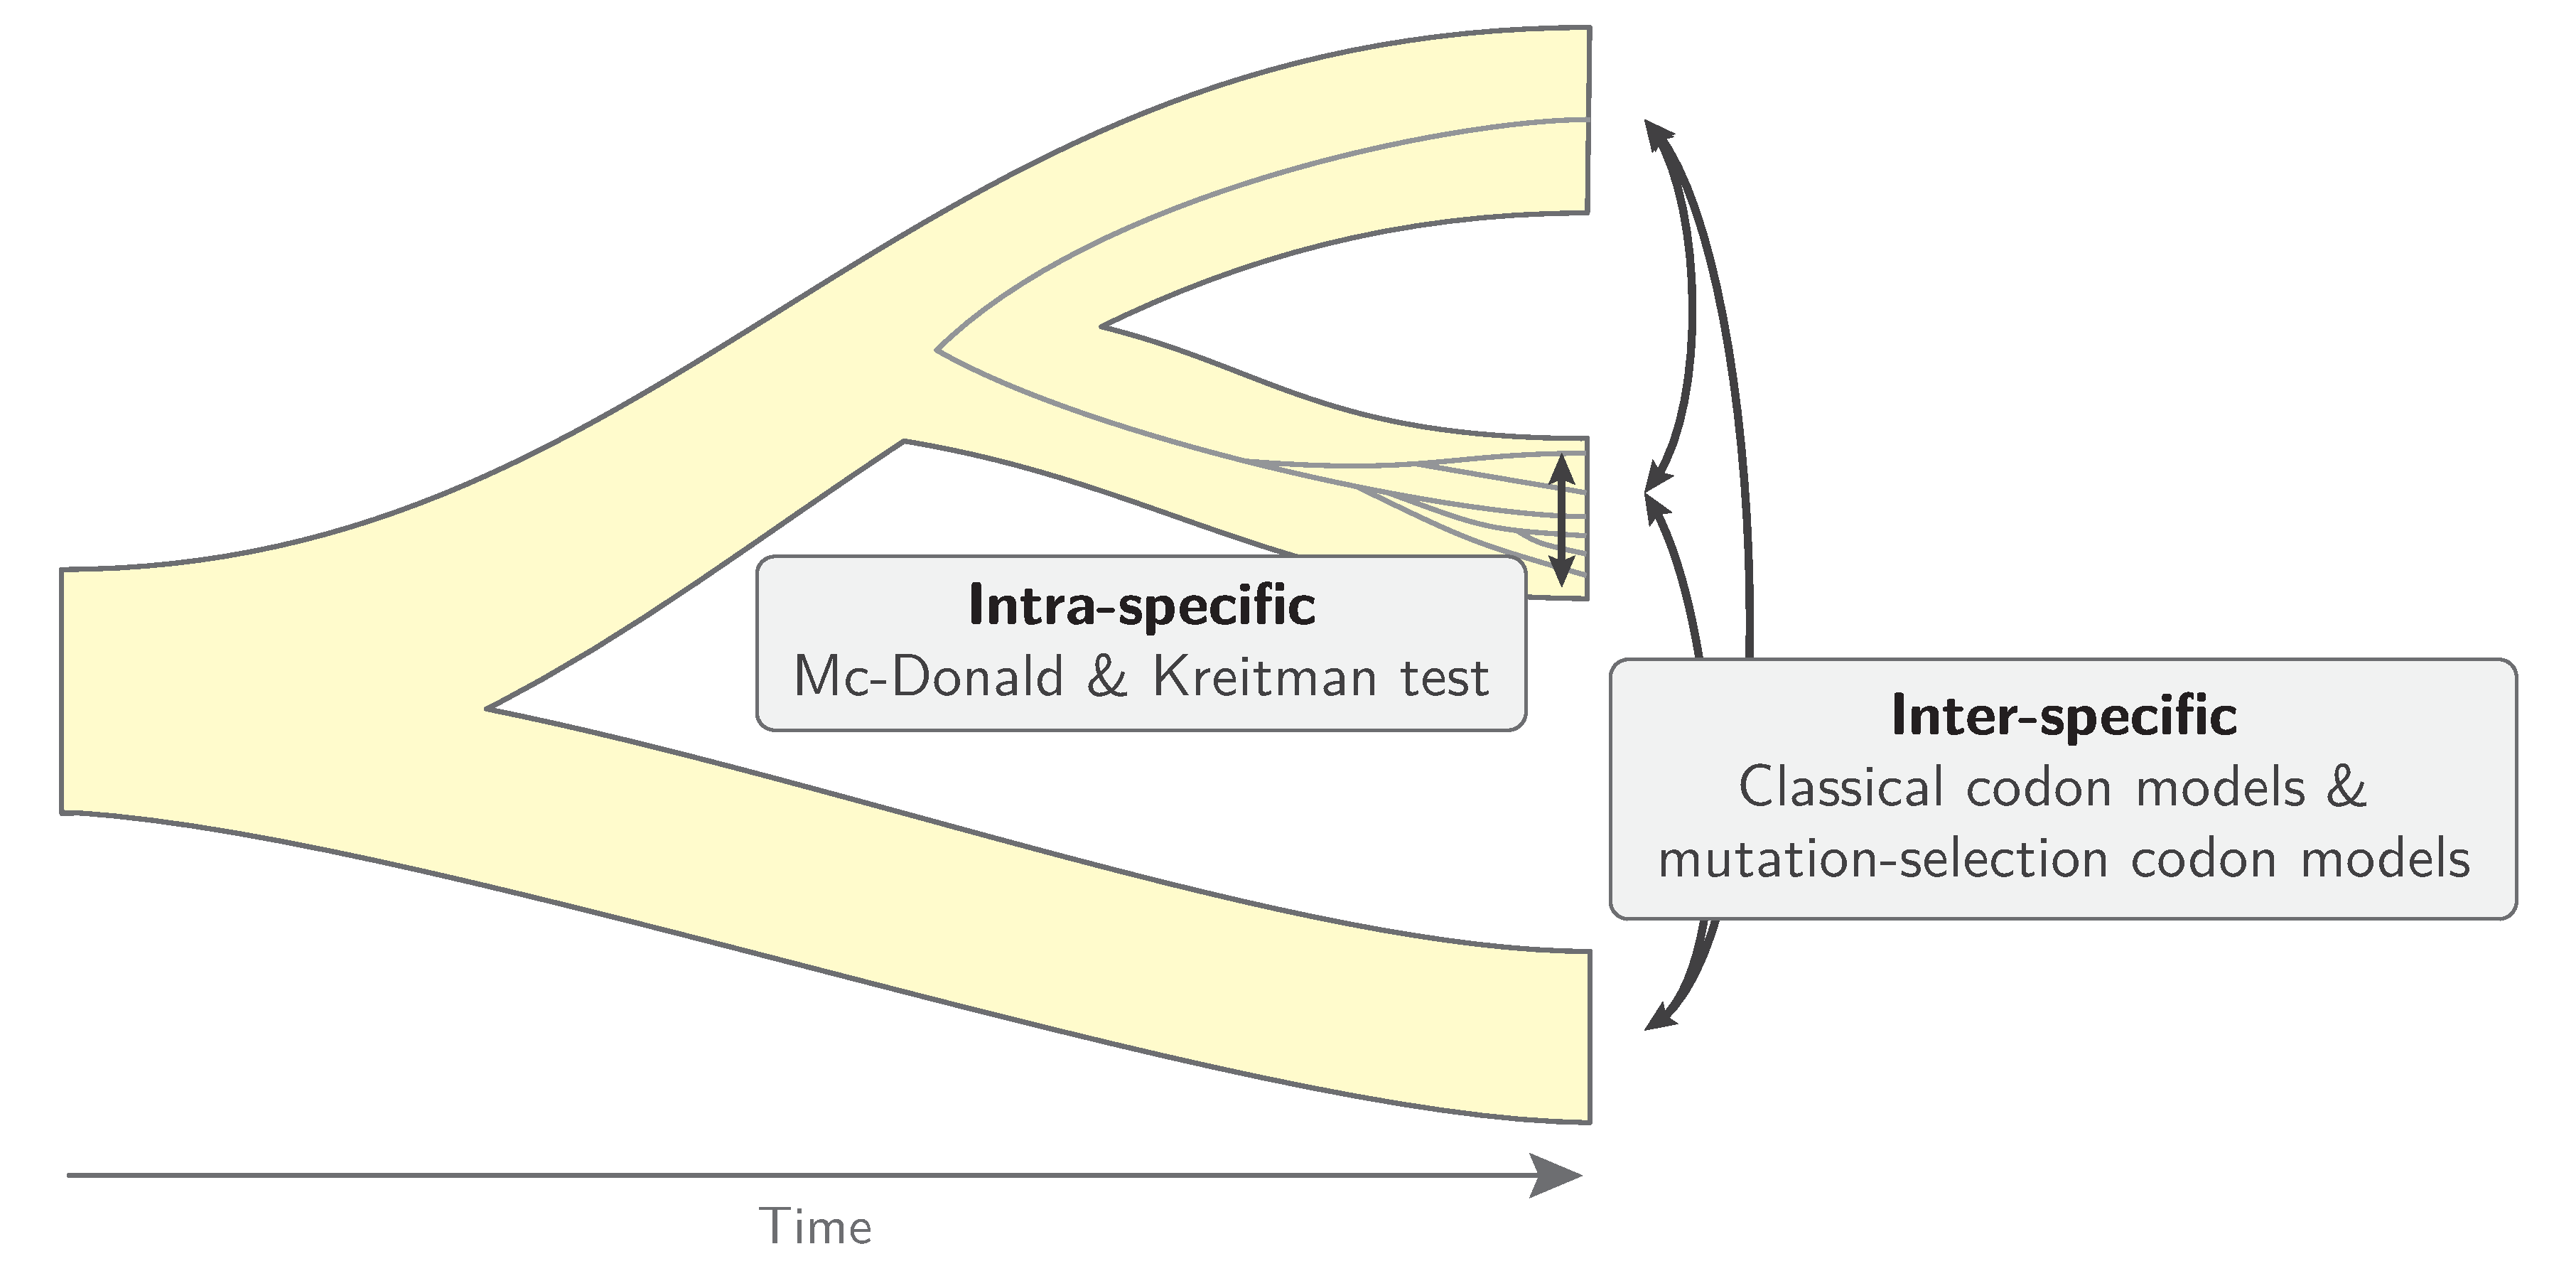
\includegraphics[width=\textwidth] {figures/inter-intra}
	\caption{Detecting adaptive evolution in coding sequences from inter- and intra-specific data}
\end{figure}

$\bullet$ From the availability of divergence and polymorphism data, it is now possible to ask whether the rate of non-adaptive evolution measured by phylogenetic mutation-selection models matches the rate estimated from SFS.
Are phylogenetic codon models and population-genetics models independently estimating the same parameters?

\section{Unifying phylogenetic and population-genetics model}
\label{sec:unifying-phylogenetic-and-population-genetics-model}

$\bullet$ Along this manuscript, polymorphism inside species has not been leveraged. Can we unify phylogenetic and population-genetics model?

$\bullet$ Selection is more easily detectable in substitution, while mutation bias is more easily detectable in polymorphism (SFS).
Unless they are carefully articulated, see chapter \ref{chap:NucleotideBias}.
Hence to disentangle the gBGC for example, integrated phylogenetic and population-genetics methods should be devised.

$\bullet$ Also, the availability of intra-specific diversity across taxa, allow to align orthologous protein coding DNA sequence across and within species.

$\bullet$ Example of integration between phylogeny and population genetics in the context of a DFE in \citet{Wilson2011}.

$\bullet$ Example of integration using scaling properties of the evolutionary process~\citep{DeMaio2013, Schrempf2016, Bergman2018, Schrempf2019} able to disentangle gBGC and mutational bias~\citep{Borges2019, Borges2020}.

$\bullet$ Because mechanistic codon models are based on population-genetics first principles, they can theoretically be extended to account for within taxa diversity.

$\bullet$ The strategy can be to augment molecular divergence data between species with information about molecular polymorphism within species.

$\bullet$ Such attempt has been tried during the first year of the PhD, where the formalism, based on Poisson Random fields can be found in appendices page \pageref{sec-appendix:PRF}.
The methods has found to be rather straightforward to implement into BayesCode, extending mutation-selection formalism.

$\bullet$ First, it was found to be computationally intensive, even though optimizing the computation with sufficient statistics.
Secondly, the method provided sensible estimation of diversity ($\theta = 4 \Ne u$) based on generated simulation under Wright-Fisher model of evolution (SimuPoly).
Most importantly, the assumption of constant drift along the phylogeny assumed by mutation-selection codon models was arguably the strongest assumption to relax in such context.
In other words, why integrating polymorphism and diversity in extant species if $\Ne$ is considered constant along the phylogeny.
It was historically the reason to extend phylogenetic site-specific mutation-selection codon models by incorporating branch-specific $\Ne$ presented in chapter \ref{chap:MutSelDrift}.

$\bullet$ After extending mutation-selection with branch specific drift, we actually realized that the susceptibility of substitution rate to changes in $\Ne$ is too strong because of site-independence assumption (chapter \ref{chap:GenoPhenoFit}), effectively amortizing the range of $\Ne$ which could be inferred.

$\bullet$ Hence, even tough site- and branch-specific mutation-selection phylogenetic codon models can be extended by incorporating signal of polymorphism, which actually has been implemented in Bayescode (-p option).

$\bullet$ Based on these observations, I believe it is not yet the path forward to build an unified phylogenetic and population-genetics model.

\section{Mechanistic and phenomenological models}
\label{sec:mechanistic-and-phenomenological-models}

$\bullet$ In order to reduce the complexity of mechanistic models, analytical models could allow to relate microscopic parameters of protein coding sequences to macroscopic parameters of evolution in a similar fashion of chapter \ref{chap:GenoPhenoFit}.
Subsequently, the microscopic parameters can be inferred from divergence and polymorphism data, and compared to their experimental estimation.

$\bullet$ The methodology can be found in \citet{Brevet2019}.

\section{Reproducible science}
\label{sec:reproducible-science}

I argue that analytical models, computational simulations and inference models are complementary, but more importantly they are necessary to each others.
Theoretical modeling allow to understand the principles, simulations allow to verify the soundness.
Inference allow to extract and test the theoretical results using empirical data.
Simulations have a dual role, testing the robustness of both inference procedures and theoretical results, outside of their comfort zone and assumptions.
However, this assume we are confident enough to write reproducible computations, as such the next section is dedicated to my personal experience and take away.

First, I stand firmly on the ground that data, codes and scripts should be rendered open-access of any published and peer reviewed paper.
Practically, the availability of the data and source code should simply be enforced upon submission to journal, which is currently not the case for all journals, even in bio-informatics and genomics fields.
It is true that such enforcement bears the consequence to weight more burden on scientists upon publishing.
However, it avoids the bloating of technical debt, or research debt where we build on the ground of a dangerous and possibly shaky basement.
It encourages peer collaboration, both helping the team or person whom made the code available, and the community as a whole.
A straightforward way is to provide a \textit{git} versioned repository, with the advantage that collaboration is facilitated trough web hosted repository such as GitLab (hosted by institutions) or GitHub (hosted by Microsoft).

Nonetheless, code availability is a necessary condition, but not the sole requirement of reproducible research.
Specific instructions to reproduce the results should also be made available, where many tools are available to this aim~\citep{Wilson2014,Darriba2018}.
The first step necessary to reproduce a code is to have the required environment, meaning the necessary libraries and dependencies of the code and scripts.
For script and code written in Python, the package manager anaconda (or conda) provides a straightforward environment to configure the necessary libraries with their versions.
More complex environment requiring code compilation or system-level packages can leverage containerization technology such as Docker or Singularity for example, but any other containers implementing system-level virtualization is very helpful to provide the necessary libraries.
Once the environment is specified, the documentation can be made available as a README with the necessary instructions.
More generally, notebooks such as \textit{Jupyter Notebook}, \textit{RMarkdown} or \textit{org-mode} to name a few also provide an environment knitting together code and instructions, allowing to follow step-by-step experiments, analysis and results, in a similar fashion as laboratory notebook which are strictly required in wet labs.
It is important to note that notebooks can run code from a variety of languages (C++, Haskell, Java, Julia, Python, Wolfram Language, Matlab, Ruby, ...).
These tools are emerging in the community, as well as Workflow management system (Nexflow, Snakemake, etc) allowing to create reproducible and scalable data analyses running on computing clusters.

Using this range of tools helps other scientists which might want to understand, test or build upon published works.
Moreover, they are also very helpful for the person or team implementing them since a more rigorous and reproducible environment allows to more easily track down bugs and test programs under different conditions or dataset\footnote{Notebooks are very useful to present work and data analysis, but should not be used during development since they often offers poor integration with debugger and code inspection tools, enforce awkward software design patterns, and often result in bloated versioned repository.}.
During the development period, continuous integration pipelines are valuable to increase the reliability of code generation, which should be used whether working alone or inside team, but is of course more critical for collaborative code where one cannot control all the code written.
Collaborative coding practices such as peer-coding sessions is really useful to implement critical code at the core of the program under development.
I argue that the efficiency peer-coding sessions is provided by dividing the tasks into a group focused in the detailed implementation while the others a free to focus on edge cases and the overall implication of different implementations.
Moreover, peer-coding sessions provides a convenient and structured place for learning good practices, for expanding its technical knowledge while pruning bad habits.
An other remarkable practice is to write two independent version of the program, using if possible different algorithm and languages but with the same functionality, but most importantly by a different person.
Then testing the program against each others on the same conditions and dataset should result in the same outcome\footnote{An extreme version is adversarial coding (or chaos engineering), where the goal is to find conditions on which the adversary program fails.}.
Such model of reproducible computing experiment and analysis is laborious and demanding, but I argue this is the definition of reproducibility we collectively should aim for, namely where one can independently reproduce the same experiment, and if reproducibility fails one can run the code with different conditions to pinpoint the failing code (which might actually be in both versions).
Personally, having practiced this method I strongly believe it pervasively reduces our research debt that we might inadvertently burden other with whenever not realizing the program is bugged, and ultimately save us time on debugging and research conduction.
Finally, explaining to others our choices of algorithms, implementation and data structure requires us to express intelligibly our mental ideas and therefor better understand them, while gaining from others insight and algorithmic expertise.

\section{Concluding remarks}
\label{sec:concluding-remarks}

$\bullet$ This work is modest attempt to construct integrated models of protein coding DNA sequences evolution.

$\bullet$ It succeeded in consolidating the idea that the patterns of substitutions inform us on long term fluctuation of drift along branches, and selection along sites.

$\bullet$ It did not succeeded in modeling the fitness landscape, apparently either too site-specific, or integrated over too many sites.
It is an indication that fitness landscape of protein coding sequences is between this two extremes.

$\bullet$ It is building block to bridge phylogeny and population-genetic, constructing an integrated framework is theoretically possible but with limited scope.
However, confronting the estimation of phylogenetic codon and population-genetics, through for example the proportion of adaptive substitution is a path forward to build bridges.

$\bullet$ Finally, I believe this thesis is not providing any ground breaking, nor disruptive results, but instead is consolidating the theoretical models on which molecular evolution is based, and points out the pitfall to avoid.
Science is alike a mutation selection process not optimized but as to trade off exploration of new ideas and exploitation of old ones.
Attempts to build bridges and connexion between fields, alike recombination, can bring the best of both worlds but many attemps are required.